\documentclass{article}
\usepackage[utf8]{inputenc}
\usepackage{graphicx}
\usepackage{caption}



\title{Search Algorithms: A Graphical Summary}
\author{Seth Kirby}
\date{September 2014}

\begin{document}

\maketitle

\section{Overview}
\noindent%
\begin{minipage}{\linewidth}
\makebox[\linewidth]{
  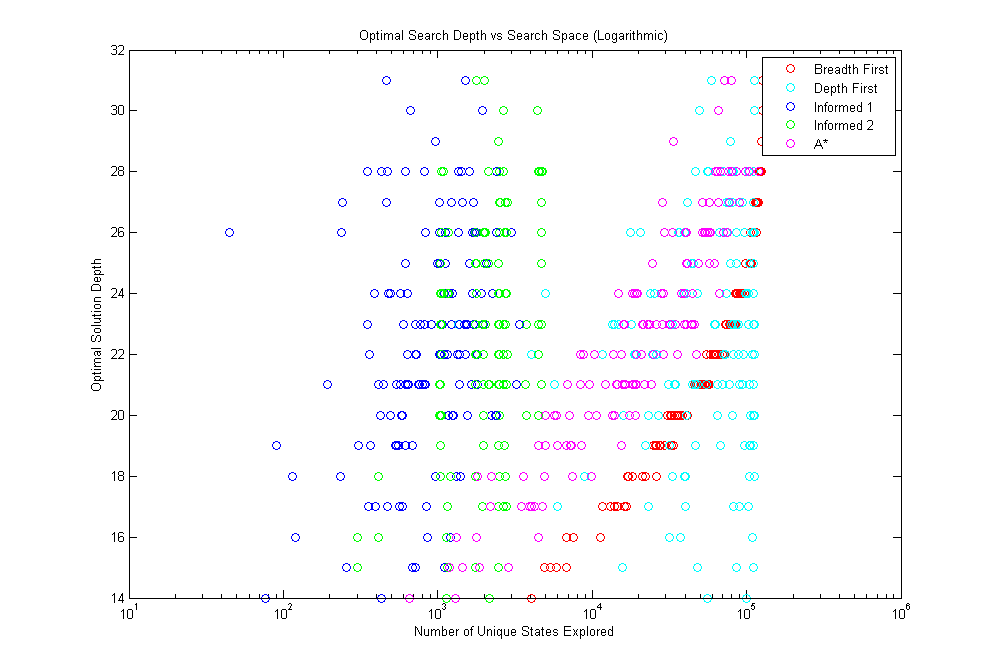
\includegraphics[keepaspectratio=true,scale=0.5]{2}}
\captionof{figure}{An logarithmic overview of solution depth and unique state exploration of the 8 puzzle across BFS, DFS, Best First Search with Hamming distance, Best First Search with integer representation, and A* with Hamming Distance.  Logarithmic on both axes.}\label{visina8}
\end{minipage}

Depth first features a parabolic curve, as it explores until it cannot create unique states, and only then decreases the depth of solution as it backs out and digs into the stack.

Breadth first and A* look fairly similar, minimizing solution depth at the cost of increased state exploration when compared to either implementation of best first.  The implementation of A* used for this example will not give the optimal solution, as it uses combined Hamming distance as a heuristic.  The Hamming distance of each state in an exploration chain is summed to score the priority queue, so A* in this example is providing the optimal Hamming minimized result.

Generally, best first using hamming distance provides better results than integer representation, minimizing unique state exploration, while producing a lower solution depth.  Best first with integer representation produces an interesting clustering effect, as states are compared via integer distance representation (with 123456780 representing the goal state), solution states are grouped into distinct cliffs of unique state exploration totals.  Generally integer representation distance provides a working heuristic, but results in solutions tending to be found in discrete units of work.

\section{Search Depth and Search Space}


\noindent%
\begin{minipage}{\linewidth}
\makebox[\linewidth]{
  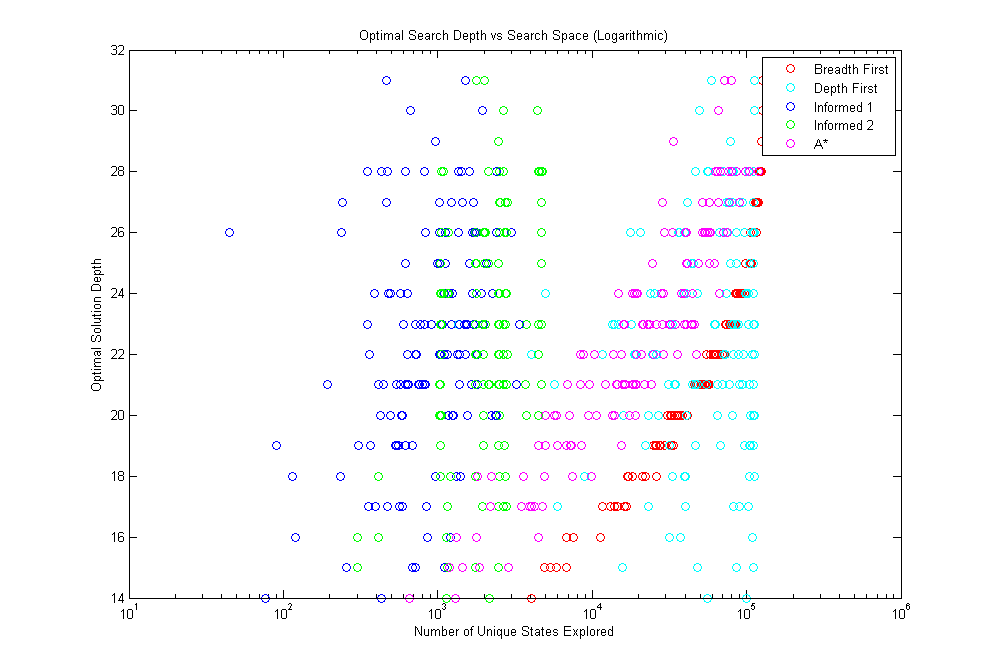
\includegraphics[keepaspectratio=true,scale=0.5]{2}}
\captionof{figure}{A comparison of the unique state exploration of all search strategies when compared to the optimal solution depth provided by BFS.  Logarithmic on the X axis.}\label{visina8}
\end{minipage}

\noindent%
\begin{minipage}{\linewidth}
\makebox[\linewidth]{
  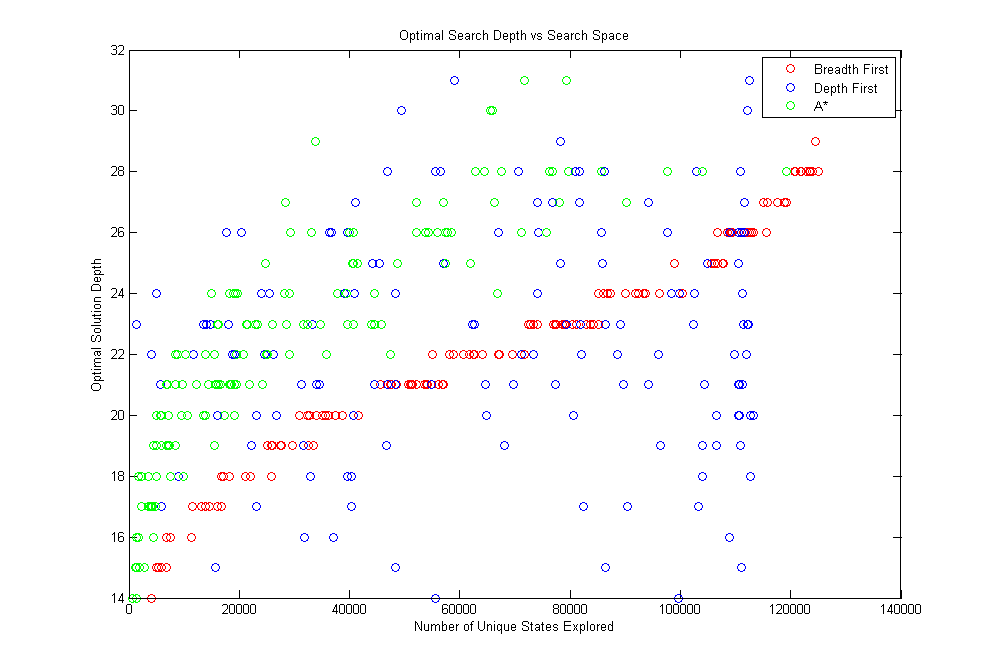
\includegraphics[keepaspectratio=true,scale=0.5]{3}}
\captionof{figure}{BFS state exploration is very tightly linked to optimal solution depth.  A* is less linked, while never performing worse than BFS.  Depth first is very loosely linked.}\label{visina8}
\end{minipage}

\noindent%
\begin{minipage}{\linewidth}
\makebox[\linewidth]{
  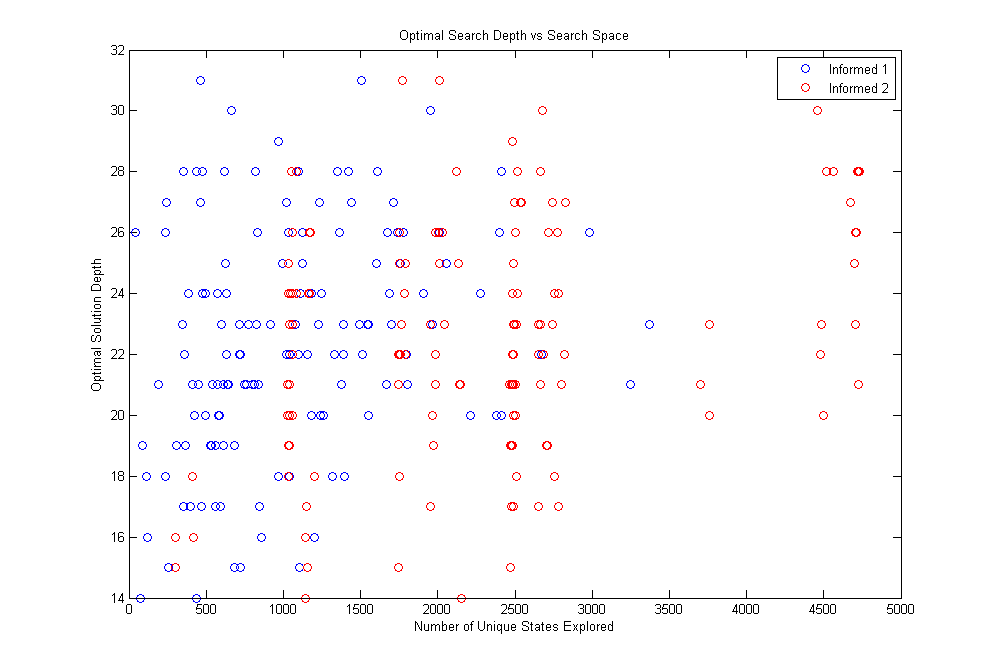
\includegraphics[keepaspectratio=true,scale=0.5]{4}}
\captionof{figure}{Best first using Hamming distance is the best performing, while we are better able to see the unique solution state cliffs of best first with integer representation.}\label{visina8}
\end{minipage}

\section{Branching and Search Space}

\noindent%
\begin{minipage}{\linewidth}
\makebox[\linewidth]{
  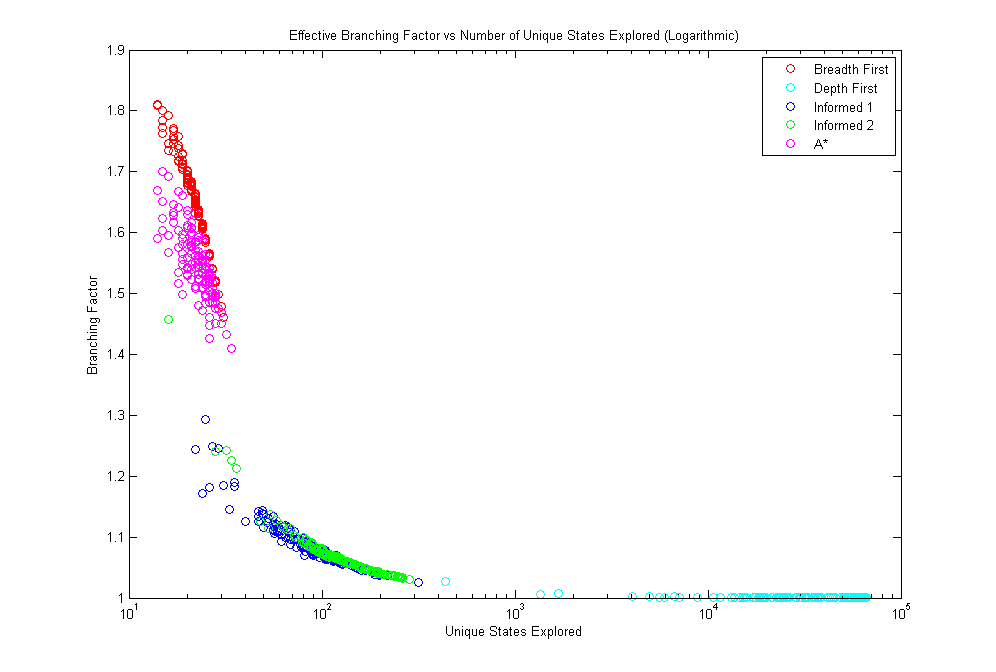
\includegraphics[keepaspectratio=true,scale=0.5]{5}}
\captionof{figure}{A comparison of branching factor across search strategies.  Logarithmic on the X axis.}\label{visina8}
\end{minipage}

Breadth first has the highest branching factor, as searches exhaustively through its vicinity before pushing the horizon forward.  Depth first has the lowest branching factor, as it generally will find a deep solution, with a very high number of moves, but little deviation from the trunk.  The branching factor for depth first rises slightly if no solution is found before exhausting options near the trunk.  A* branches slightly less than breadth first due to intelligent node selection.  Both informed searches have similar branching factors, fewer explored states using Hamming as a heuristic.

\noindent%
\begin{minipage}{\linewidth}
\makebox[\linewidth]{
  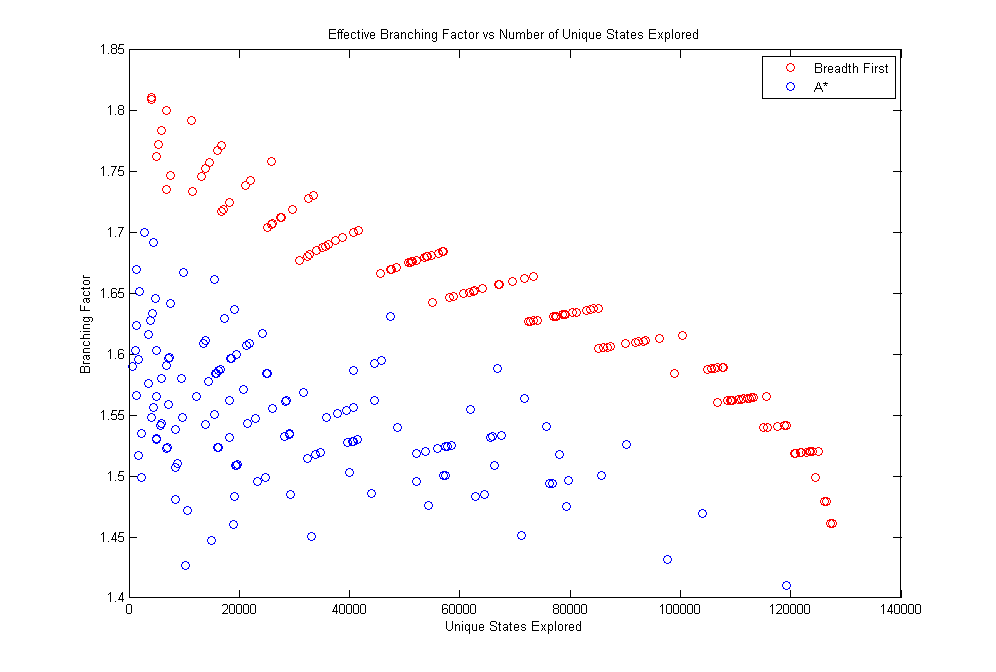
\includegraphics[keepaspectratio=true,scale=0.5]{6}}
\captionof{figure}{Branching factors of BFS and A*.  Note the striations that occur strongly in BFS due to the progressive nature of exploration, an effect less prominent though apparent in A*.}\label{visina8}
\end{minipage}

\noindent%
\begin{minipage}{\linewidth}
\makebox[\linewidth]{
  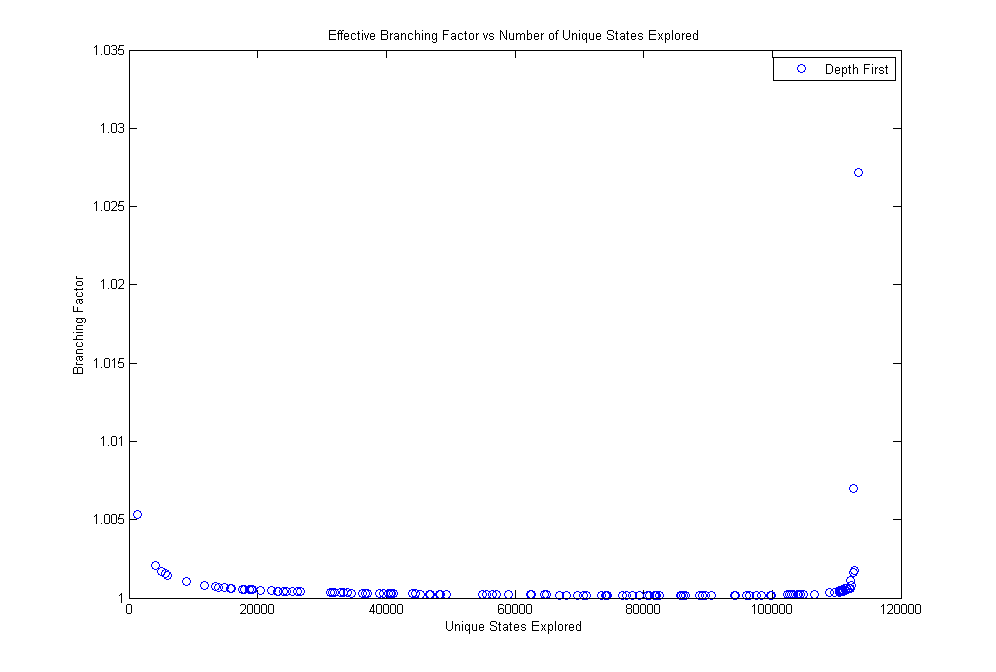
\includegraphics[keepaspectratio=true,scale=0.5]{8}}
\captionof{figure}{Branching factor of DFS.  Note the rising branching factor on the tail of state exploration.}\label{visina8}
\end{minipage}

\noindent%
\begin{minipage}{\linewidth}
\makebox[\linewidth]{
  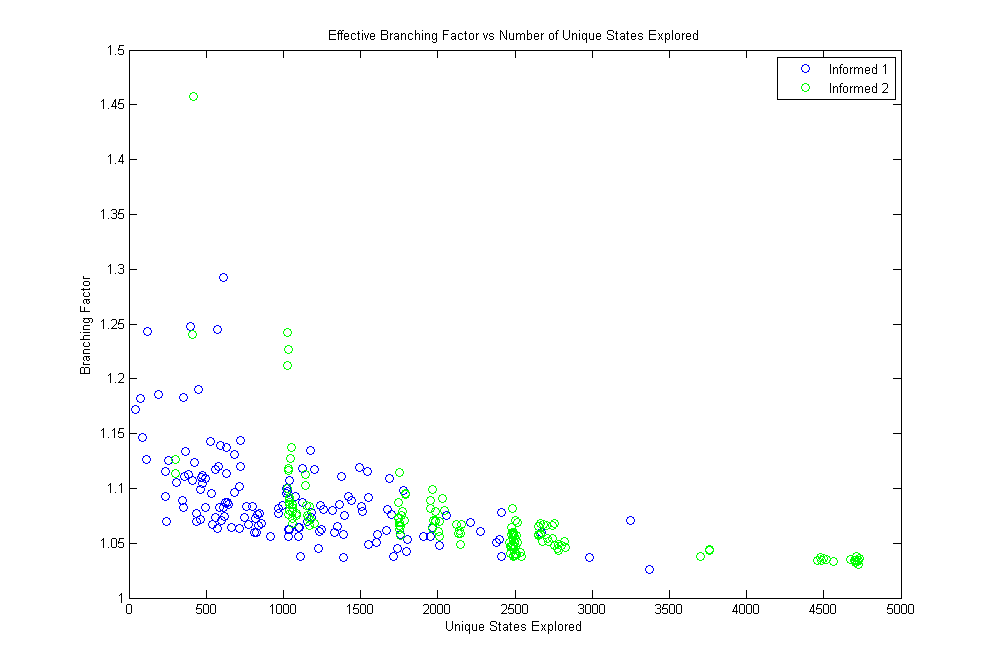
\includegraphics[keepaspectratio=true,scale=0.5]{7}}
\captionof{figure}{Branching factors of best first search.  Note again the clustering that occurs with representation integer difference comparison.}\label{visina8}
\end{minipage}

\end{document}
